\documentclass[12pt,a4paper,twoside,openany]{report}

\usepackage[utf8]{inputenc}
\usepackage[francais]{babel}
\usepackage[T1]{fontenc}
\usepackage[left=2cm,right=2cm,top=2cm,bottom=2cm]{geometry}
\usepackage{graphicx}
\usepackage{palatino, euler} 
\usepackage[colorlinks=true,linkcolor=blue,urlcolor=blue]{hyperref}
\usepackage{fancyhdr}
\usepackage{lastpage}
\usepackage{float}
\usepackage{ulem}

\urlstyle{sf} % style des url
\setlength{\parskip}{2ex plus .4ex minus .4ex} % espacement vertical entre les paragraphes
\setlength{\headheight}{15.6pt}
\uchyph=0 % empêcher la coupure des mots commençant par une majuscule
\setlength{\fboxsep}{3mm}
\renewcommand{\tabcolsep}{0.5cm} % padding dans les tableaux
\renewcommand{\arraystretch}{1.5} % padding dans les tableaux

% Encadré
\newcommand\encadre[1]{\vspace{1.5ex}\fbox{\begin{minipage}{0.92\textwidth}\begin{center}#1\end{center}\end{minipage}}\vspace{2.5ex}}

\newcommand{\titre}{Copier pour mieux créer} % Copier pour mieux coller / Copier, c'est le progrès / Copier pour mieux créer
\newcommand{\moi}{David Sferruzza}
\author{\moi}
\title{\textit{\titre}}
\date{décembre 2012}

% Entête et pied de page
\fancyhf{}
\lhead{{\footnotesize \leftmark}}
\lfoot{\moi}
\rfoot{\thepage/\pageref*{LastPage}}
\renewcommand{\footrulewidth}{0.1pt}
\pagestyle{fancy}

% Entête et pied de page pour les 1ères pages des chapitres
\fancypagestyle{plain}{
	\lhead{}
	\chead{}
	\rhead{}
	\renewcommand{\headrulewidth}{0pt}
}

\begin{document}

\maketitle

\begin{titlepage}
~\vfill
\begin{center}
\begin{minipage}[c]{10cm}
\begin{center}
	\textbf{\titre}
	\linebreak
	\linebreak
	\moi\\
	\textbf{david.sferruzza@gmail.com}
	\linebreak
	\linebreak
	2012
	\linebreak
	\linebreak
	\linebreak
	
\includegraphics[scale=.05]{images/copyleft.png} 
	\end{center}
	\textit{Copyleft} : cette oeuvre est libre, vous pouvez la copier,
	la diffuser et la modifier selon les termes de la
	\textit{Licence~Art~Libre}~---~\url{http://www.artlibre.org/}
\end{minipage}
\end{center}
\vfill
\end{titlepage}


\tableofcontents

\chapter*{Introduction}
\addcontentsline{toc}{chapter}{Introduction} 

\begin{quote}
{\Large \textit{<<~Le piratage, c'est du vol !~>>}}
\end{quote}

C'est ce qu'on entend de nos jours lorsque l'on va voir un film au cinéma.
Avertissements du FBI sur nos DVD, condamnations des <<~pirates~>> à de fortes amendes, protections anti-copie : la culture se porte mal.
C'est le discours que les médias nous tiennent, et c'est ce qui est en train de devenir une vérité pour la plupart d'entre nous.

Pourtant, les chiffres tiennent un tout autre discours : l'industrie de la culture engrange chaque année davantage de bénéfices.
On voit sortir dans nos salles de cinéma des \textit{blockbusters} de plus en plus gigantesques en terme de budget et de nombre d'entrées.

Ce qui est sûr, c'est que ces dernières décennies ont été riches en terme d'innovations technologiques, notamment dans les moyens de communication, avec la prolifération des ordinateurs et d'internet.
Il est maintenant très facile d'échanger des informations, de les copier, et de les stocker.
L'éloignement géographique est de moins en moins un problème, et chaque créateur peut espérer une visibilité à la hauteur de son talent.

Mais alors qu'en est-il vraiment ?
La copie incarnée par internet va-t-elle détruire la créativité et dénaturer la culture tout en mettant au chômage ceux qui l'alimentent ?
Ou alors est-ce l'invention majeure de notre temps : celle qui réduira les inégalités et répandra le savoir à travers le monde ?

Passionné de nouvelles technologies, de cinéma et de jeux vidéo, j'observe depuis plusieurs années ce problème se muer en combat, et peut-être bientôt en guerre.
Aujourd'hui, j'ai décidé d'essayer de tirer cette histoire au clair.
Je suis convaincu que nous sommes à l'aube de changements majeurs dans nos sociétés, et il est de notre devoir de citoyens de nous assurer que ces changements convergent bien vers l'obtention d'un monde \textbf{meilleur} pour \textbf{tous}.

Mon objectif ici est d'apporter une vision globale de la situation, des choses qui sont en jeu, et des moyens d'actions dont nous disposons.

Mon discours s'organisera en trois étapes.
Je reviendrai d'abord sur les notions de bases qui entourent et rassemblent l'action de copier et celle de créer.
Ces mécanismes sont importants en tant que socle et centre du problème en même temps.
Je décrirai ensuite la position actuelle de la société vis à vis de la copie, et j'insisterai sur l'incohérence de cette position.
À partir de là, il sera plus facile de comprendre les enjeux de la situation, pour aborder la 3\ieme{} partie : les pistes pour un monde meilleur.

\chapter{La copie, est-ce que ça mord ?}

\begin{quote}
\textit{{\Large <<~Inventer en toute chose, c'est vouloir mourir à petit feu ; copier c'est vivre.~>>} \hspace{25pt}Honoré de Balzac -- \underline{Pierre Grassou}}
\end{quote}

\section{Qu'est-ce que la copie ?}

Le terme <<~copie~>> peut prendre plusieurs sens. Je ne vais pas parler ici de copie dans le sens <<~une feuille de copie~>>. Je parle de copie dans le sens <<~duplication~>>.

Voici les trois premières définitions du mot <<~copie~>> trouvées dans le dictionnaire\footnote{\textbf{NOM DU DICO}} :
\begin{enumerate}
\item Reproduction exacte d'un écrit, du contenu d'un texte, d'une bande magnétique ; double, duplicata.
\item Reproduction d'une œuvre, d'un objet d'art, en principe par les mêmes techniques que celles de l'original ; réplique.
\item Imitation, calque.
\end{enumerate}\bigskip

La première chose qu'on peut remarquer, c'est que si la première définition est très claire quant au caractère <<~exact~>> de la copie, les deux définitions suivantes restent vagues sur cet aspect.
L'autre point, c'est que ces définitions n'incluent pas le sens moderne de la copie, à savoir la copie de données numériques (qui est au cœur de notre sujet).

Durant les dernières décennies, l'humanité a assisté à l'avènement de la donnée numérique : il est devenu possible, sous réserve de pouvoir l'exprimer de manière discrète, de stocker n'importe quelle information sur des supports numériques.
Outre leur capacité de stockage bien plus élevée que les moyens traditionnels, ces supports présentent l'avantage de pouvoir être lus et écrits rapidement, et pour un coût insignifiant.
On qualifie les informations et les œuvres placées sur de tels supports <<~d'immatérielles~>> ou de <<~dématérialisées~>>, car le support (l'objet, qui est matériel donc) est dissocié des données qu'il contient.

En couplant ça avec la prolifération d'Internet, il devient possible de copier des données sans avoir à se déplacer, ni payer un coût variable important, comme le prix du papier lorsque l'on veut dupliquer un livre par exemple.
Bien sûr, il y a un coût : les infrastructures qui supportent et constituent Internet, ainsi que les terminaux des utilisateurs ont besoin d'énergie pour fonctionner.
Mais ce coût est tout de même faible par rapport aux coûts de duplication d'un livre, et peut être en grande partie considéré comme un coût fixe, c'est à dire ne dépendant pas de la quantité de données qu'on veut copier.

Par ailleurs, il se pose la question de la nuance entre copie conforme et inspiration : à partir de quand peut-on dire qu'il y a copie et non inspiration ?
Cette question est très complexe.
On peut cependant imaginer quelques réponses possibles.
On pourrait dire qu'il y a copie lorsqu'un auteur présente comme sienne une œuvre strictement identique à une œuvre existante.
Pourtant, si on copie l'ensemble d'une œuvre, mais qu'on en modifie un détail, on considérera pourtant 	que l'œuvre obtenue a été copiée.

On pourrait, au contraire, dire qu'il y a copie lorsqu'on utilise dans une œuvre tout ou partie d'une autre œuvre, pour peu que les éléments importés n'aient pas été modifiés.
Mais on voit rapidement la limite de cette définition : y a-t-il toujours copie lorsqu'on parle d'éléments importés d'autres œuvres, mais si petits et élémentaires qu'on ne saurait identifier l'œuvre dont ils proviennent ?
Même si le résultat apparaitrait comme inspiré d'autres œuvres, il n'en resterait pas moins que l'auteur a procédé par copie pour obtenir certains éléments de son œuvre.
Le cas inverse est également envisageable : obtenir le même résultat qu'un autre, mais sans avoir eu connaissance des travaux de ce dernier.

Comme je le disais, la différence entre copier et s'inspirer n'est pas simple à exprimer.
La difficulté est de placer une limite claire et concrète, qui permet de démontrer qu'on se trouve dans un cas et pas dans l'autre.
Mais finalement, est-t-il utile de faire cette distinction ?

%(définition, différence avec inspiration)
\section{Créer implique copier ?}

Commençons par le commencement et posons-nous la question : que signifier <<~créer~>> ?
En guise de réponse, voici trois éléments d'une définition\footnote{Source : \url{https://fr.wiktionary.org/wiki/créer}} :

\begin{enumerate}
\item Tirer quelque chose du néant, faire de rien quelque chose.
\item Donner l'existence à quelque chose qui n'existait pas encore, éventuellement à partir d'autres éléments.
\item Imaginer, inventer.
\end{enumerate}\bigskip

D'après les exemples associés à ces définitions, la première serait utilisée pour désigner <<~créer~>> dans le sens religieux du terme uniquement.
Les deux autres définitions semblent être plus proches des domaines que nous étudions ici.

Il semble possible de créer à partir de rien, principalement dans deux cas : en étant un dieu, ou en imaginant.
Je ne développerai pas ici la première possibilité, car elle fait référence à un débat qui, pour le moment, nous dépasse tous.

Par contre, il semble tout à fait possible théoriquement de créer à partir de rien grâce à notre imagination.
On pourrait même dire que c'est le propre des mathématiques :

\begin{quotation}
\textit{<<~Les mathématiques se distinguent des autres sciences par un rapport particulier au réel.
Elles sont de nature purement intellectuelle, fondées sur des axiomes\footnote{Un axiome désigne une vérité indémontrable qui doit être admise} déclarés vrais (c'est-à-dire que les axiomes ne sont pas soumis à l'expérience, même s'ils en sont souvent inspirés) ou sur des postulats provisoirement admis.~>>}\footnote{Source : \url{https://fr.wikipedia.org/wiki/Mathématiques}}
\end{quotation}

Cependant, même dans le domaine des mathématiques, le réel et l'existant ont de l'importance.
En effet, de nombreux créateurs\footnote{Pas seulement mathématiciens ou même scientifiques} utilisent leur imagination pour mettre en scène des choses existantes, de manière à catalyser leur créativité.

Par exemple, Henri Poincaré, grand mathématicien français, décrit une démarche scientifique en quatre temps : préparation, incubation, illumination et vérification.
Si la première et la dernière étape relèvent beaucoup de la technique et de la méthode, les phases d'incubation et d'illumination sont en grande partie de l'ordre de l'imaginaire.
De nombreux mathématiciens\footnote{Notamment Wendelin Werner, Jacques Hadamard et Cédric Villani ; source : Sciences Humaines \no{}221} confirment que, lors de ces étapes de <<~recherche~>>, créer des images et des univers mentaux mettant en scène des idées, éléments et objets connus est une stratégie quasiment indispensable. La construction de la représentation mentale serait même indissociable de la résolution.

On peut même aller encore plus loin dans l'illustration de la nécessité de s'inspirer du réel dans la démarche de création scientifique : les expériences de pensées.
Voici donc une histoire mettant en scène Galilée, célèbre savant italien du 16\ieme{} siècle.
À savoir qu'il existe d'autres histoires connues très similaires impliquant Albert Einstein ou James Clerk Maxwell, mais celle de Galilée est, à mon sens, la plus facile à réaliser soit même\footnote{Ami lecteur, je compte sur toi ;)}.

Tout le monde connait l'expérience de Galilée qui aurait laissé tomber deux objets du haut de la tour de Pise, l'un étant plus lourd que l'autre, pour montrer que les deux objets touchent le sol au même instant.
Cette expérience contredit la physique aristotélicienne : Galilée cherche à montrer que la vitesse de la chute des objets dans le vide est indépendante de leur masse.
Sauf qu'au début, cette expérience ne s'est jamais déroulée ailleurs que dans l'imagination de Galilée !

Dans sa représentation mentale de la tour de Pise, il a supposé que la masse la plus lourde allait toucher le sol avant l'autre.
Il s'est ensuite dit, que s'il attachait les deux objets ensemble, le plus léger allait ralentir le plus lourd, et donc que celui-ci toucherait le sol après un temps plus long.
Mais comme les deux masses sont attachées ensemble, on peut aussi considérer qu'elles forment une seule masse, plus importante que chacune des deux masses prises séparément.
Cette masse devrait donc, en suivant le postulat de départ, arriver au sol après un temps plus court !
Cette contradiction permet de réfuter l'hypothèse de départ, et mène à la conclusion qu'on connait.

L'expérience a, bien sûr, eu lieu de nombreuses fois par la suite ; et la loi de la chute des corps dans le vide fut confirmée.
Mais c'est imaginer un univers similaire à celui qu'il connaissait qui a permis à Galilée d'attendre la phase <<~d'illumination~>>.

Là où je veux en venir, c'est qu'à part le cas, finalement très rare, voire impossible, où on crée à partir de \textbf{rien}, créer implique à un moment ou un autre s'inspirer de ce qu'on connait, qui existe déjà.
Et qui dit <<~inspiration~>> dit\dots{} copie !

C'est la thèse que défend Kirby Ferguson, un réalisateur New-Yorkais, dans son film en quatre parties : \textbf{Everything Is A Remix}\footnote{À voir absolument ! \url{http://www.everythingisaremix.info/watch-the-series/}}.

\encadre{
\center
Selon lui, voici les éléments fondamentaux de la créativité :\\
\vspace{10pt}
{\LARGE Copy, Transform, Combine}\\
\textit{Copier \hspace{34pt} Transformer \hspace{34pt} Combiner}\\
\vspace{10pt}
{\Huge =}\\
\vspace{10pt}
{\LARGE Remix}
}

Pour lui, toute création est un remix de créations existantes, qu'on a donc copiées, transformées (ou adaptées), et enfin combinées.
Il n'hésite pas à donner des exemples, dans une conférence TED\footnote{\url{http://www.ted.com/talks/kirby_ferguson_embrace_the_remix.html}}, la plupart étant issus du domaine de la musique.
Ainsi, il fait écouter des chansons de Bob Dylan et les chansons dont elles ont été <<~inspirées~>>.
On constate sans trop d'efforts que certains aspects (paroles, sons, ...) sont très similaires.

Un autre exemple, dans le domaine du cinéma cette fois-ci, est \textbf{Kill Bill}.
L'épopée vengeresse en deux parties de Quentin Tarantino est aujourd'hui considérée comme un des exemples les plus marqués de remix\footnote{La preuve en images : \url{http://vimeo.com/19469447}}, à tel point qu'elle en devient un hommage à toute une période cinématographique.

Les exemples ne manquent pas, parfois même de l'aveu de leurs créateurs !
Au hasard : lorsque George Lucas s'est lancé dans le projet qui deviendra par la suite \textbf{Star Wars}, il voulait à la base faire un \textit{remake} du Flash Gordon des années 30.
N'étant pas en position légale pour faire ça, il du faire évoluer son idée ; le Star Wars tel qu'on le connait comporte tout de même bon nombre de similitudes avec Flash Gordon, et rentre très bien dans la définition du remix que nous venons de voir.

L'idée que tout est un remix va bien plus loin que le domaine de la culture, et n'est pas ancrée dans notre époque. Gutenberg, connu pour avoir inventé l'imprimerie à caractères mobiles, s'est inspiré de techniques et de solutions existantes :

\begin{table}[H]
\center
\begin{tabular}{c|c}
Presse à imprimer & 1440 apr. J.-C. \\
\hline
Caractère mobile & 1040 apr. J.-C. \\
Presse à vis & 1 apr. J.-C. \\
Encre & 180 av. J.-C. \\
Papier & 1800 av. J.-C.
\end{tabular}
\caption{Les technologies nécessaires à l'invention de l'imprimerie}
\end{table}

Plus récent, et tout aussi connu, Henry Ford n'a pas inventé la chaine d'assemblage (1867), ni les pièces interchangeables (1801), ni l'automobile (1885).
Mais il a su combiner tous ces éléments en 1908 pour produire la première voiture en quantité industrielle : la Ford Model T.
Ainsi, il déclare :

\begin{quotation}
\textit{<<~I invented nothing new.
I simply assembled the discoveries of other men behind whom were centuries of work.
Had I worked fifty or ten or even five years before, I would have failed.
So it is with every new thing.
Progress happens when all the factors that make for it are ready, and then it is inevitable.
To teach that a comparatively few men are responsible for the greatest forward steps of manking is worst sort of nonsense.~>>}
\end{quotation}

Ce qui donne en Français :

\begin{quotation}
\textit{<<~Je n'ai rien inventé de nouveau.
J'ai simplement assemblé les découvertes d'autres hommes qui portaient derrière elles des siècles de travail.
Si j'avais travaillé cinquante, dix ou même cinq ans plus tôt, j'aurais échoué.
Il en va de même pour chaque nouvelle invention.
Le progrès se produit quand tous les facteurs qui le rendent possible sont là ; ensuite, il devient inévitable.
Dire que relativement peu d'hommes sont responsables des plus grandes avancées de l'humanité est le pire des non-sens.~>>}
\end{quotation}

Tous ces exemples montrent que la copie est une action indispensable dans le processus de création.
On a pourtant tendance à la juger de manière péjorative.
Mais nous y reviendrons\dots{}

J'aimerais terminer cette partie en te demandant, ami lecteur, comment as-tu appris écrire ?
J'imagine que tu as commencé par recopier des lignes de lettres.
Et comment apprend-on à jouer de la musique ?
En jouant des morceaux écrits par des musiciens célèbres.
Tu sais programmer ?
Beaucoup de personnes (dont moi même) ont commencé en copiant/collant des extraits de code sources.

La copie est aussi une action fondamentale pour qui veut apprendre.
Peu importe le domaine, il y a toujours une phase d'apprentissage par la copie, avant d'avoir acquis suffisamment de lucidité pour pouvoir s'en émanciper.
Plus on devient compétant dans un domaine, plus on est capable de transformer et de combiner.
Mais la copie, l'inspiration, de matériaux existants est inéluctable.

%(everything is a remix, images mentales, apprentissage, exemple de l'imprimerie, exemple de Ford)
\section{Copier n'est pas voler}

(rareté vs abondance, copier = multiplier, propriété)

\chapter{Interdire la copie, ou l'encourager : l'incohérence du système actuel}

Nous avons vu dans le chapitre précédent que la copie est une action naturelle que nous exerçons tous tout à long de notre vie.
Cependant, la société ne se positionne pas forcément dans ce sens, et prend une position incohérente par rapport à la copie.
Nous allons voir pourquoi dans ce chapitre.

\section{Brevet et droit d'auteur}

Nous n'allons pas aborder de manière exhaustives les notions de brevet et de droit d'auteur, car ce sont des notions complexes qui touchent beaucoup de domaines, et qui varient en fonction du pays étudié.
Je vais par contre tâcher de les définir de manière suffisante pour pouvoir les intégrer à notre réflexion sur la copie.
Sauf si je le précise explicitement, je parlerai surtout en me basant sur la législation française.

Commençons par le droit d'auteur (ou son équivalent américain, le <<~copyright~>>).
<<~Le droit d'auteur est l'ensemble des prérogatives exclusives dont dispose un auteur ou plus généralement ses ayants droit (société de production, héritiers) sur des œuvres de l'esprit originales.~>>\footnote{Source : \url{https://fr.wikipedia.org/wiki/Droit_d\%27auteur}}

Ici, on parle donc bien <<~d'œuvres de l'esprit~>>, donc immatérielles.
Bien souvent, ces idées vont être matérialisées, et placées sur des supports (papier, DVD, \dots{}) dont on ferra commerce.
Le problème, c'est que ce modèle est lucratif pour ceux qui fabriquent les objets (libraires et imprimeurs, dans l'exemple du livre) ; il n'y a finalement pas de raison spontanée première pour que ceux-ci décident de rémunérer les auteurs des œuvres qu'il exploitent.

L'idée du droit d'auteur c'est de dire que si on fait commerce de la matérialisation de l'œuvre de quelqu'un, on lui doit un pourcentage.
La démocratisation de ce mécanisme en France est souvent attribuée à Beaumarchais, qui, en temps que dramaturge, voulait toucher un pourcentage sur la recette perçu par les comédiens qui jouaient ses pièces.

On peut diviser le droit d'auteur en deux branches :
\begin{itemize}
\item \textbf{le droit moral}, qui reconnaît à l'auteur la paternité de l'œuvre et qui vise aussi le respect de l'intégrité de l'œuvre ;
\item \textbf{les droits patrimoniaux}, qui confèrent un monopole d'exploitation économique sur l'œuvre, pour une durée variable (selon les pays ou cas) au terme de laquelle l'œuvre entre dans le domaine public \textit{(nous reviendrons sur la notion de domaine public en même temps que l'explication sur les brevets)}.
\end{itemize}\bigskip

L'auteur peut jouir de ces deux droits automatiquement, dès le moment où il a créé une œuvre.
Le droit d'auteur était à la base prévu pour durer un maximum de 5 ans.
De nos jours, on parle plutôt de 70 ans après la mort de l'auteur !

On peut déjà entrapercevoir les limites d'un tel système : à partir de quand une œuvre de l'esprit, une idée, peut être appartenir à quelqu'un ?
Comme je l'ai argumenté dans le premier chapitre, il est difficile de s'approprier quelque chose d'immatériel dans le sens où cette chose n'a souvent pas de limite clairement identifiable.
D'un autre côté, ce système est une solution qui a été trouvée pour nourrir les artistes qui produisent des œuvres immatérielles.

Cependant, on constate de plus en plus de cas où le droit d'auteur est utilisé pour protéger l'artiste contre son public (parfois même à l'insu de l'artiste), chose pour laquelle il n'a pas été prévu du tout à la base.
Mais nous y reviendrons par la suite\dots{}

L'autre <<~entrave~>> à la copie est le brevet (ou son équivalent américain, le <<~patent~>>).
<<~Un brevet est un titre de propriété industrielle qui confère à son titulaire non pas un droit d'exploitation, mais un droit d'interdiction de l'exploitation par un tiers de l'invention brevetée, à partir d'une certaine date et pour une durée limitée (20 ans en général).~>>\footnote{Source : \url{https://fr.wikipedia.org/wiki/Brevet}}

Contrairement au droit d'auteur qui est automatique, il faut faire une demande pour obtenir un brevet, ce qui a un coût (très important pour un particulier).
Un brevet n'est valable que dans un État donné.
Il est cependant possible de déposer un brevet auprès de plusieurs États, mais le coût en est multiplié et sa validation n'est pas assurée partout, car les organismes de validations sont indépendants (certains organismes peuvent délivrer des brevets valables dans plusieurs États).
Les brevet sont plutôt réservés aux inventions et aux techniques industrielles.

Pour être brevetable, une invention doit correspondre à trois critères :
\begin{enumerate}
\item Elle doit être nouvelle, c'est-à-dire que rien d'identique n'a jamais été accessible à la connaissance du public, par quelque moyen que ce soit (écrit, oral, utilisation\dots{}), où que ce soit, quand que ce soit. Elle ne doit pas non plus correspondre au contenu d'un brevet qui aurait été déposé mais non encore publié.
\item Sa conception doit être inventive, c'est-à-dire qu'elle ne peut pas découler de manière évidente de l'état de la technique, pour un homme du métier.
\item Elle doit être susceptible d'une application industrielle, c'est-à-dire qu'elle peut être utilisée ou fabriquée dans tout genre d'industrie, y compris l'agriculture (ce qui exclut les œuvres d'art ou d'artisanat, par exemple).
\end{enumerate}\bigskip

Il est également exigé que la description complète de l'invention et de la manière de la reproduire doit être incluse dans le brevet, de manière à ce que le contenu technique soit disponible lors de la publication de la demande, et le reste après la fin de validité du brevet.

En effet, l'objectif premier du système de brevet est d'encourager les créateurs et inventeurs à partager leurs avancées avec le reste de la communauté.
Le problème qui se pose est que si une entreprise développe un produit et décide de le vendre, elle n'est pas à la l'abri qu'une autre entreprise récupère son produit et le vende également, mais bien moins chère car n'ayant pas de frais de recherche et développement à couvrir.
Le brevet permet de partager sa création avec la communauté, mais de conserver l'exclusivité sur son exploitation (ou sur qui peut l'exploiter) pendant une durée suffisante pour rembourser les frais de recherche et développement.
Une fois cette durée écoulée, la création tombe dans le domaine public.

On appelle <<~domaine public~>> l'ensemble des biens intellectuels qui ne sont plus protégés par le droit d'auteur ni par un brevet.
Les éléments issus du domaine public peuvent être utilisés par n'importe qui, à n'importe quelle fin, sans que l'auteur ou les ayants droit puissent faire valoir un quelconque droit d'exclusivité.

Il est très important d'avoir un domaine public conséquent et bien alimenté, car ce sont les technologies qui s'y trouvent qui serviront de fondations aux inventions de demain.
Le domaine public favorise donc le progrès, mais surtout un progrès équitable, dans le sens où les technologies qui s'y trouvent sont exploitables par tout le monde, et pas seulement par une poignée d'élus.

%(historique, définition, objectifs)
\section{L'industrie du droit d'auteur}

Malheureusement, les systèmes du droits d'auteur et du brevet commencent à atteindre leurs limites et ne sont plus en phase avec l'ère du numérique.
On voit apparaitre une industrie du droit d'auteur, qui détourne les buts originels de ces systèmes dans le but de faire toujours plus de profit.

Le terme <<~industrie du droit d'auteur~>> en dit déjà long : il ne s'agit plus du droit d'auteur en tant que moyen mais en tant que fin !
On s'éloigne du concept <<~le droit d'auteur me permet d'amortir ma phase de recherche et développement~>> pour aller vers <<~le droit d'auteur me permet une exclusivité et une rente pour une durée de l'ordre de ma vie entière~>>.

Une des formes de cette industrie du droit d'auteur est les <<~patent trolls~>> ainsi que leurs homologues, les <<~copyright trolls~>>.
Les patent trolls sont des entreprises créées dans le seul but d'acquérir un portefeuille de brevet et d'attaque en justice d'autres entreprises dont les produits violeraient ces brevets.
Les copyright trolls fonctionnent de manière similaire.

Ces sociétés peuvent être très agressives, allant parfois jusqu'à faire du lobbying pour faire pencher en leur faveur la législations relative au système des brevets et du droit d'auteur.
Par exemple, on peut voir dans le graphique suivant que la durée d'application du droit d'auteur, après la mort de ce dernier, en France n'a fait qu'augmenter au cours des derniers siècles.
L'espérance de vie ayant aussi augmenté, on a, de nos jour, une durée théorique maximale moyenne du droit d'auteur d'environ 150 ans ! Et des lois sont à l'étude pour étendre encore une fois cette durée\dots{}

\begin{figure}[H]
\center
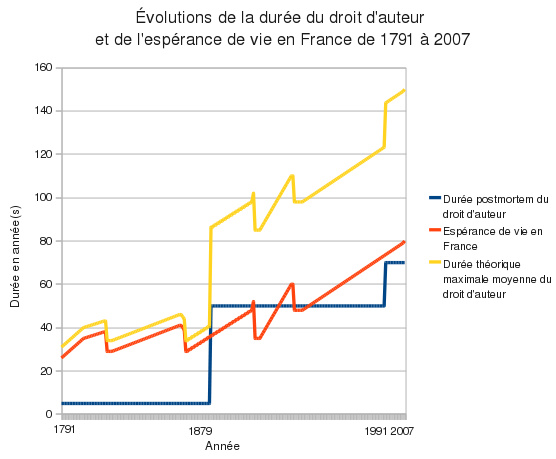
\includegraphics[scale=.85]{images/duree_du_droit_d'auteur_en_France_depuis_1791.png}
\caption{Évolution de la durée du droit d'auteur en France}
\end{figure}

Ces sociétés peut scrupuleuses font également appel à des méthodes d'intimidation pour faire toujours plus de profit.
L'astuce est de menacer d'attaquer en justice, pour violation du droit d'auteur/brevet détenu par la compagnie, des petites entreprises ou des particuliers.
Ceux-ci se voient alors offrir une porte de sortie, pour régler le différent <<~à l'amiable~>> : bien souvent le paiement d'une somme importante, mais moins importante et <<~risquée~>>\footnote{Risquée, car cette somme peut évoluer en fonction du verdict} que des frais de justice.
Il peut s'agir d'un coup de bluff, car le copyright/patent troll n'est pas obligé d'être sûr de gagner en justice : il lui suffit juste de le faire croire et d'intimider sa victime suffisamment pour que celle-ci choisisse d'elle même de régler ce différent fictif à l'amiable.

De telles entreprises sont un fléau pour la société, car elles cherchent à produire de la richesse en violant le système, mais surtout en obstruant la création !
C'est une des raisons pour lesquelles les systèmes du brevet et du droit d'auteur atteignent leurs limites : la société se retrouve à rémunérer la non-valeur ajoutée, ce qui est contraire à beaucoup de ses principes.

Dans le même ordre d'idées, certains n'hésitent pas à déposer des brevets tellement vagues ou évidents qu'ils peuvent alors potentiellement attaquer n'importe qui en justice pour violation de brevet.
Voici par exemple du smiley, issue du site \href{http://copyrightmadness.tumblr.com/}{CopyrightMadness} :

\begin{quotation}
\textit{<<~En Finlande, un troll de premier ordre a tenté d'enregistrer comme marque\dots{} le smiley.
Vous avez bien lu : la petite binette souriante de côté dont vous ponctuez vos tweets et vos emails ;-)
Fort heureusement, les juges qui avaient été saisis de cette demande ont estimé que les smileys ne pouvaient pas faire l'objet d'une telle protection et qu'ils devaient rester d'usage libre pour tous, y compris à des fins commerciales.
Un peu de Trademark Wisdom, ça fait du bien de temps en temps, mais sachez qu'en France, le smiley (la face jaune souriante, pas les signes typographiques) fait bien l'objet d'une protection, accordée à la famille Loufrani, qui en fait un usage particulièrement délirant :-(~>>}\footnote{Source : \url{http://storify.com/Copyrightmad/copyright-madness-du-1er-au-7-octobre}}
\end{quotation}

En parallèle de ces cas <<~extrêmes~>>, les entreprises qui, elles, produisent de la valeur n'hésitent pas non plus à utiliser le système à leur avantage, et, encore une fois, au désavantage du progrès et de la société.

On peut par exemple citer Apple, qui a décidé de breveter un concept, utilisé dans son iPhone, qu'on peut résumer par : <<~déverrouiller son téléphone en glissant son doigt sur une icône~>>.
Il parait complètement fou que ce brevet de 28 pages puisse exister et appartenir à quelqu'un.

Ce cas n'est pas isolé.
Un diagramme qui schématise les actions en justice pour violation de brevet dans le domaine des smartphones de 2008 à 2012 est disponible en annexe (page \pageref{annexe-smartphones}).

On peut voir que Apple est très impliqué dans ce genre d'affaires, que ce soit en tant que victime ou qu'agresseur.
Peu avant sa mort, Steve Jobs (co-fondateur et dirigeant de Apple pendant une longue période), a déclaré, à propos d'Android (système d'exploitation pour mobiles, principal concurrent du système pour iPhone, iOS) :

\begin{quote}
\textit{{\Large <<~I'm going to destroy Android, because it's a stolen product.
I'm willing to go thermonuclear war on this.~>>}}
\end{quote}

Ou, en français :

\begin{quote}
\textit{{\Large <<~Je vais détruire Android, car c'est un produit volé.
Je déclencherais une guerre thermonucléaire s'il le faut.~>>}}
\end{quote}

C'est à mettre en relation avec le fait que Apple ait copié les prototypes de Xerox, sans quoi nous ne connaitrions probablement même pas l'entreprise à la pomme.
En effet, la plupart des mécanismes que nous utilisons aujourd'hui sur n'importe quel ordinateur grand public ont été inventés par Xerox : souris, bureau, dossiers et fichiers, menus déroulants, \dots{}
En parlant de ça, Steve Jobs cite Picasso :

\begin{quote}
\textit{{\Large <<~Les bons artistes copient, les grands artistes volent.
~>>}
\begin{flushright}Pablo Picasso\end{flushright}}
\end{quote}

Si Xerox avait réagit comme Apple et ses concurrents réagissent de nos jours, nul doute que cette compagnie plus grande et plus mature n'aurait fait qu'une bouchée d'un Apple jeune et inexpérimenté\dots{}

%(copyright/patent troll, rémunération du non-ajout de valeur, appropriation d'idées communes, exemple Apple)
\section{Une histoire qui se répète ?}

Ces démonstrations d'agressivité et ces répressions à l'encontre des technologies de copie et de partage de l'information ne sont pas nouvelles.
Je vais survoler ici quelques exemples issus du passé, et nous verrons si l'Histoire peut nous enseigner une leçon.
Pour de plus amples détails, je recommande le 3\ieme{} chapitre (si ce n'est l'ensemble) du document <<~Sur la réforme du droit d'auteur~>>\footnote{\url{http://reformedroitauteur.sploing.fr/}}, sur lequel je me baserai pour écrire cette partie.



%(exemples de "crises" similaires et résolues, exemple des bibliothèques)
\section{Interdire implique contrôler} % ou L'interdiction implique le contrôle
(DRM, HADOPI, DPI, cloud, vie privée, annexe vélo)
\section{Partager favorise le progrès}
% sanctionner copie = sanctionner inspiration (cf chap 1)
(les pirates achètent, exemple de Arduino, exemple de la mode)

\chapter{À l'abordage du futur}

Si la copie est indispensable à la création et que la société cherche de plus en plus à la punir, sommes-nous condamnés à devoir courir le risque d'un procès à chaque fois que nous créerons quelque chose ?
Je pense que nous pouvons éviter cette situation, et je vais donner des pistes qui vont dans ce sens.

\section{Ne pas devenir esclave du progrès}

Comme je l'ai montré dans la partie \ref*{drm} (page \pageref{drm}), les moyens de contrôle de la copie se sont démocratisés, et avec eux la fonte de certaines de nos libertés fondamentales et d'une partie de notre vie privée.
Mais il n'est pas trop tard pour réagir \dots{}
Avant de poursuivre cette réflexion, je vais devoir expliquer un certain nombre de nouvelles notions.

Commençons par la licence d'une œuvre.
Pour faire simple, lorsqu'un créateur produit une œuvre, il peut définir une licence (ou <<~contrat de licence~>>).
Il s'agit un contrat légal qui explique les conditions d'utilisation de l'œuvre, auquel chaque utilisateur doit se plier.

Pour un logiciel, on peut par exemple avoir une licence de type commercial, qui interdit complètement l'utilisation du logiciel sans avoir payé une redevance, ou alors une licence dite <<~freeware~>> qui permet l'utilisation de ce dernier de manière gratuite.

La particularité pour un logiciel est que, dans la plupart des cas, on peut distinguer deux composantes :

\begin{itemize}
\item son code source : c'est ce que le développeur va écrire dans un langage de programmation donné ; il s'agit d'un ensemble de fichiers textes ;
\item son exécutable : il s'agit d'une traduction du code source en langage machine, obtenue par l'action dite de <<~compilation~>> ; l'exécutable est incompréhensible par un humain et on ne peut pas l'utiliser pour récupérer le code source !
\end{itemize}

Pour faire une analogie, disons que le code source est une recette de gâteau ainsi que ses ingrédients, et que l'exécutable est le gâteau lui-même.
Grâce au pâtissier, il est possible d'obtenir un gâteau à partir de sa recette et de ses ingrédients.
Par contre, il ne sera pas possible de récupérer ni la recette ni les ingrédients à partir du gâteau !
On pourra éventuellement récupérer quelques ingrédients qui n'auraient pas été mélangés (comme les petites fraises présentes sur le glaçage) et un bon pâtissier pourra sans doute réécrire une partie de la recette ; mais il ne lui sera pas possible de récupérer tous les ingrédients et la recette exacte !

Certains créateurs distribuent le code source de leur logiciel, on dit alors que le logiciel est <<~libre~>> ou <<~open source~>>.
D'autres ne le font pas et distribuent uniquement l'exécutable.
Leur logiciel est alors dit <<~propriétaire~>> ou <<~privateur~>>.

La notion de logiciel libre a été formalisée en 1983 par Richard Stallman, créateur de la Free Software Foundation\footnote{\url{https://www.fsf.org}}.
La définition d'un logiciel libre est basée sur quatre libertés :

\begin{enumerate}
\item[0.] la liberté d'exécuter le programme, pour tous les usages ;
\item la liberté d'étudier le fonctionnement du programme et de l'adapter à ses besoins ;
\item la liberté de redistribuer des copies du programme (ce qui implique la possibilité aussi bien de donner que de vendre des copies) ;
\item la liberté d'améliorer le programme et de distribuer ces améliorations au public, pour en faire profiter toute la communauté.
\end{enumerate}

Certains logiciels propriétaires peuvent donner les libertés \no{}0 et \no{}2 à l'utilisateur, mais rendent les deux autres libertés inaccessibles puisqu'ils ne distribuent pas leur code source.

Au delà de l'aspect légal, le logiciel libre est une philosophie.
Il s'agit de rendre le contrôle à l'utilisateur : il a les moyens d'étudier le programme qui va s'exécuter sur son matériel, et de le modifier s'il ne lui plait pas.
Cette possibilité de pouvoir étudier le fonctionnement d'un logiciel peut paraitre inutile pour le commun des mortels, qui ne connait pas la programmation, mais c'est pourtant quelque chose de très important !

Plus un logiciel libre a du succès, plus des utilisateurs avancés vont (statistiquement) l'étudier.
Si ce logiciel contient des mécanismes nocifs pour l'utilisateur (DRM, récolte et envoi de données personnelles, etc.) ou des failles de sécurité pouvant nuire à l'utilisateur, alors un signal d'alarme est tiré, et le logiciel incriminé va devoir revoir sa copie ou sera soigneusement évité par la communauté.

Ceci assure que presque l'intégralité des logiciels libres prennent soin de la sécurité et de la vie privée de l'utilisateur.
Les utilisateurs de logiciels propriétaires doivent quant à eux faire confiance aux auteurs du logiciel pour toutes ces questions.
Quand il s'agit de logiciels édités par des entreprises, dont le but est par définition de faire du profit, on peut se demander si c'est bien placer sa confiance \dots{}

La différence entre le libre et l'open source est principalement une différence de philosophie.
Le logiciel libre met en avant la liberté qu'il apporte à ses utilisateurs, tandis que le logiciel open source va apprécier la communauté de développeurs qui va se former autour de lui et lui permettre de se développer plus efficacement.
En pratique, presque tous les logiciels libres correspondent à la définition d'un logiciel open source et inversement.

Pour ne pas avoir à réécrire à chaque fois un nouveau contrat de licence pour leurs nouvelles créations, les développeurs de logiciels libres ont tendance à récupérer des textes de licences existantes (qui la plupart du temps sont libres eux aussi).
Certaines licences sont donc très répandues parmi les logiciels libres.
On peut citer, par exemple, la GNU General Public License\footnote{Écrite par Richard Stallman lui-même, pour son projet GNU} (GNU GPL) ou la licence MIT\footnote{Du nom de l'université qui l'a créée (Massachusetts Institute of Technology)}.

La licence MIT donne à toute personne recevant le logiciel le droit illimité de l'utiliser, le copier, le modifier, le fusionner, le publier, le distribuer, le vendre et de changer sa licence, à la seule condition que les noms des auteurs soient cités, même en cas de modification du logiciel.
La licence GNU GPL offre des droits similaires, à la différence qu'elle met en œuvre la notion de copyleft\footnote{Il s'agit d'un jeu de mot basé sur le mot <<~copyright~>> ; l'idée de copyleft est opposée à celle de copyright}, ce qui veut dire que le logiciel doit être redistribué avec la même licence, même s'il a été modifié.

\begin{quotation}
\begin{flushright}
\textit{<<~L'idée centrale du copyleft est de donner à quiconque la permission d'exécuter le programme, de le copier, de le modifier, et d'en distribuer des versions modifiées - mais pas la permission d'ajouter des restrictions de son cru. C'est ainsi que les libertés cruciales qui définissent le logiciel libre sont garanties pour quiconque en possède une copie ; elles deviennent des droits inaliénables.~>>}
\begin{flushright}Richard Stallman\end{flushright}
\end{flushright}
\end{quotation}

Les logiciels libres permettent donc de ne pas devenir esclaves du progrès, car ils donnent le pouvoir aux utilisateurs, et non pas à leurs créateurs comme c'est le cas pour les logiciels propriétaires.
Les logiciels sont déjà partout, pas seulement dans nos ordinateurs, et il nous revient de choisir si nous voulons garder le contrôle sur notre technologie, ou le confier à des sociétés dont le but est de faire du profit.

Il est facile de faire ressentir ce besoin du logiciel libre contre l'esclavage grâce au domaine médical\footnote{Un autre exemple que celui que je vais développer ici est disponible à cette adresse : \url{http://www.framablog.org/index.php/post/2012/11/26/un-coeur-gros-comme-ca}}.
Il existe actuellement un bon nombre d'appareils médicaux dont le fonctionnement est régit par des logiciels (par exemple, les stimulateurs cardiaques, ou <<~pacemakers~>>).
On peut dire que ces appareils ne valent que ce que valent leurs logiciels.
Si ces logiciels sont propriétaires, il n'est pas rassurant de se dire qu'on a dans le corps des appareils dont le comportement n'est connu que par la société qui les a fabriqués.

S'ils étaient libres, ils pourraient à coup sûr bénéficier de nombreuses relectures par des experts d'horizons différents, ce qui réduirait le nombre de bogues\footnote{Francisation de l'anglais <<~bug~>> qui désigne un défaut de conception d'un programme informatique à l'origine d'un dysfonctionnement}.
Car oui, les logiciels ont des bogues.
Et lorsque ces logiciels nous maintiennent en vie, un bogue peut être fatal.
Et avec un code fermé, qu'est ce qui empêche l'appareil d'envoyer nos signaux vitaux en sans-fil à notre insu ?
Ou, s'il est nécessaire que ces informations soient envoyés en sans-fil à un autre appareil, la connexion sans-fil est-elle correctement sécurisée ?
Si ce n'est pas le cas, peut être que quelqu'un peut communiquer avec notre pacemaker et lui donner l'ordre de s'arrêter \dots{}

Le logiciel libre est un bouclier contre ce genre de pratiques et de négligences, et, en ce sens, il est indispensable.

Je vais terminer cette partie sur un dernier point : celui du patrimoine.
J'ai dit, lorsque j'ai expliqué le droit d'auteur (page \pageref{droit-auteur}), que lorsqu'on crée une œuvre de l'esprit, on se voit alors automatiquement doté de droits exclusifs relatifs à l'exploitation de cette œuvre.
Contrairement au système des brevets, qui n'offre pas de droits automatiques, le système du droit d'auteur (et du copyright) ne possède pas de base de données indiquant pour chaque œuvre son auteur, ainsi que les droits d'exploitation que celui-ci a cédé (ou pas) et à qui.

\label{oeuvres-orphelines}
Il se pose alors le problème d'œuvres orphelines, c'est à dire n'ayant pas d'auteur connu.
On ne peut actuellement pas considérer que ces œuvres font partie du domaine public, et pour cette raison, leur utilisation est un risque.

Par exemple, on peut imaginer que, voulant utiliser une œuvre dans un de mes projets, je décide de contacter son auteur pour négocier la permission d'intégrer tout ou partie de son travail dans le mien.
Ne parvenant pas à trouver cet auteur, je décide tout de même d'utiliser l'œuvre.
Quelques années plus tard, l'auteur en question réapparait, prouve qu'il est bien l'auteur de l'œuvre que j'ai utilisée, et me fait un procès pour violation du droit d'auteur.
Je perds et je dois lui payer une énorme amende.

Conclusion : une œuvre orpheline est <<~bloquée~>> entre la zone de droit et le domaine public, et l'utiliser comporte le même risque que celui d'utiliser une œuvre protégée sans l'autorisation de son 	auteur.

J'en parle ici car, pour moi, si nous ne voulons pas que les générations futures deviennent esclaves de la technologie et des idées contrôlées par une minorité, nous devons lui donner les moyens de les apprivoiser.
Et cela passe par la possibilité de ce servir des œuvres et des idées que nous allons leur léguer.
Malheureusement, le système actuel ne semble pas aller dans ce sens ; il ne tient qu'à nous de le faire évoluer, mais j'y reviendrai plus tard \dots{}

%(logiciel libre, donner le pouvoir aux utilisateurs, assurer le patrimoine, exemple du domaine médical)
\section{Partager pour mieux créer}

Comme nous l'avons vu précédemment, lorsqu'on crée, on s'inspire d'œuvres existantes, voire on les réutilise (partiellement ou intégralement).
Empêcher ce processus revient à entraver la créativité.
Mais, au contraire, le favoriser peut conduire à une créativité sans limite !

Pour cela, il faut redéfinir les lois sur la protection du droit d'auteur, mais nous en reparlerons.
L'autre possibilité est que les créateurs autorisent les autres à exploiter leurs œuvres.

On pourrait se dire que ces créateurs doivent manger, et ont donc besoin de vendre leurs œuvres.
C'est peut être vrai pour une économie de la rareté, mais, si on parle d'œuvres de l'esprit, les règles du jeu sont totalement différentes.
Il existe de nombreuses entreprises qui réussissent à vivre en publiant leur travail sous licence libre.
C'est notamment le cas de Red Hat, une société américaine éditrice de distributions Linux, qui a obtenu un chiffre d'affaire de 1 milliard de dollars américains en 2012.

Énormément de produits que nous connaissons sont basés sur des logiciels libres.
Cela veut dire que si les créateurs de ces logiciels n'avaient pas rendu libres leurs créations, aucun produit n'aurait pu se baser dessus et il aurait fallu réinventer la roue à chaque fois.

Par exemple, ma Freebox Révolution\footnote{Modem ADSL amélioré du fournisseur d'accès à Internet <<~Free~>>} embarque pas moins de 67 logiciels libres\footnote{D'après la page <<~Mentions légales~>> dans la console d'administration de la Freebox Révolution}.
Si ces logiciels n'avaient pas été libres, les développeurs de chez Free auraient du en écrire des nouveaux qui réalisaient les mêmes fonctions.
La Freebox n'aurait pas été rentable pour Free, et ne serait peut être même jamais sortie.

On peut aussi constater que Free a parfois amélioré certains de ces logiciels, probablement pour corriger quelques imperfections ou ajouter une fonction dont ils avaient besoin pour leur Freebox.
Ces modifications ont soit été publiées elles-mêmes sous licence libre, soit directement poussées vers les créateurs des logiciels concernés, dans le but que ceux-ci les intègrent à terme et en fassent bénéficier la communauté.

Cet échange de bons procédés (<<~j'utilise ton programme et en échange je partage avec toi et ta communauté les éventuelles améliorations que je lui apporterais~>>) est très courant dans le monde du libre et de l'open source.
Il ne s'agit pourtant pas d'une obligation légale : rien de tel n'est inscrit dans les contrats de licence des logiciels en question.
Il s'agit tout bonnement de créativité engendrée par le partage, et cela permet un progrès pour tous.

On peut aussi évoquer tout ce qui touche à la philosophie des hackers.
Contrairement à ce que les médias peuvent dire, le terme <<~hacker~>> n'est pas négatif.
<<~Un hacker est quelqu'un qui aime comprendre le fonctionnement d'un mécanisme, afin de pouvoir le bidouiller pour le détourner de son fonctionnement originel.~>>\footnote{Source : \url{https://fr.wikipedia.org/wiki/Hacker}}

Le hacking est une forme de créativité encore peu connue du commun des mortels.
Pourtant, de nombreuses avancées technologiques sont attribuées à des hommes qu'on pourrait qualifier de hackers.
Parfois, la curiosité pousse à aller étudier le fonctionnement d'un système donné (appareil, logiciel, voire même l'art !).
Et parfois, cette étude donne de nouvelles idées auxquelles le créateur original n'avait initialement pas pensé.
Cette approche décalée permet d'identifier des failles potentielles de sécurité qui n'auraient jamais été imaginées avec une approche <<~classique~>> de test.

Par exemple, dans les années 60, John Draper découvre un sifflet dans sa boite de céréales Cap'n Crunch.
Il se rend ensuite compte que ce sifflet est accordé sur le <<~la aigu~>>, et lui permet de reproduire la tonalité à 2600 Hz utilisée par la compagnie téléphonique Bell pour ses lignes longue distance.
Pour faire simple\footnote{Les détails sont disponibles ici : \url{https://fr.wikipedia.org/wiki/John_Draper} (et sur bien d'autres sites)}, ce sifflet lui permet de passer des appels internationaux gratuitement, grâce à une faille dans le système téléphonique.
Il fera deux mois de prison et gardera le surnom <<~Captain Crunch~>>.
Ce genre d'anecdote est amusant, mais plus courant qu'on le croit.

Il faut favoriser ces démarches de hackers\footnote{Je fais référence ici aux vrais hackers (dits <<~white hats~>>) et pas aux quelques <<~black hats~>> mal intentionnés que nous décrivent bien trop les médias} car elles ont une portée éducative, d'autant plus que l'histoire montre que c'est souvent le point de départ de nombreux progrès.
Et tout cela se met en place autour de logiques de partage.

Le phénomène <<~d'aversion à la perte~>> est une composante de la psychologie humaine.
Il fait référence à la tendance d'une personne à préférer éviter des pertes plutôt que d'acquérir des gains.
Dans notre étude, c'est, j'en suis convaincu, l'un des facteurs qui empêchent les créateurs de partager leurs œuvres.
De nombreux cas ont montré qu'il y avait souvent beaucoup plus à retirer du libre partage des œuvres que la <<~perte~>> du contrôle de ces œuvres.
Ce qui est arrivé au musicien Andy Othling illustre bien cette idée\footnote{Voir : \url{http://www.framablog.org/index.php/post/2012/10/30/ma-musique-gratuite-pendant-24h}}.

On pourrait également parler plus longuement du domaine de la mode.
Il n'y a en effet pas de copyright dans cette industrie, et pourtant elle est très rentable.
On peut même dire que c'est ce qui pousse les stylistes à créer toujours plus, sans avoir à craindre un procès parce qu'ils ont réutilisé une idée d'un concurrent.
Je ne m'étendrais pas là dessus, dans la mesure où la conférence TED animée par Johanna Blakley\footnote{\url{http://www.ted.com/talks/johanna_blakley_lessons_from_fashion_s_free_culture.html}} le fait très bien.

L'histoire montre, comme le rappelait Henry Ford (voir la citation page \pageref{ford}), que lorsque tous les facteurs qui rendent le progrès possible sont là, celui-ci devient inévitable.
On peut citer comme exemple le téléphone : le brevet concernant le téléphone fut déposé à deux heures d'intervalle par Alexander Graham Bell et Elisha Gray !
Partager, c'est s'assurer que les facteurs qui rendent le progrès possible soient là.
Nous avons besoin d'un progrès inévitable.

%(partager le plus possible, aller contre l'aversion à la perte, hacker, exemple du téléphone, exemples de réussites du libre, exemple de Arduino, exemple de la mode)
\section{Valoriser les créateurs}

Je parlais précédemment de l'affaire Megaupload.
Megaupload était un service de stockage de données dans le cloud.
Il était connu en grande partie pour sa capacité à pouvoir être utilisé comme plateforme de partage.
En effet, un utilisateur pouvait partager un lien qui permettait aux autres utilisateurs de récupérer une copie du fichier concerné.
Megaupload était donc très gênant pour les ayants droit, car il permettait aux gens de s'échanger librement des créations normalement payantes.
Cela représentait, selon eux, un manque à gagner énorme.

En janvier 2012, le FBI faisait fermer Megaupload, ou plutôt il saisit les serveurs de ce dernier qui étaient situés dans l'État de Virginie, aux États-unis.
Bien évidemment, Megaupload devint inaccessible faute de serveurs et ses utilisateurs perdirent l'accès à leurs données.
Je ne reviendrai pas sur la légitimité de cette saisie, qui se produisit dans un contexte trouble.

Ce qui m'intéresse ici c'est l'étude qui a été publiée récemment par la Munich School of Management et la Copenhagen Business School\footnote{Source : \url{http://ssrn.com/abstract=2176246}}.
Ces chercheurs allemands et norvégiens ont analysé les données hebdomadaires des cinémas dans 49 pays, de 2007 à 2012.
La conclusion est la suivante : << La fermeture de Megaupload a eu un effet négatif sur les recettes du box-office, hormis dans certains cas où l'effet été négligeable~>>.

Selon eux, Megaupload présentait un <<~effet de réseau (social) où le partage de fichiers agit comme un mécanisme pour diffuser des informations venant de personnes qui ont une volonté faible ou nulle de payer, envers des personnes qui ont une grande volonté de payer~>>.
Toujours selon eux, le cinéma d'auteur a été bien plus touché par cette fermeture que les blockbusters américains, car bénéficie d'une très faible promotion auprès des médias, et donc compte beaucoup plus sur le bouche-à-oreille.

Dans la même catégorie, l'OFCOM, l'autorité de régulation des télécoms du Royaume-Uni, a publié cette semaine une étude\footnote{Source : \url{http://www.pcinpact.com/news/75538-la-consommation-pirates-britanniques-sous-oeil-dune-etude.htm}}, menée par le cabinet Kantar Media auprès de 4 400 britanniques âgés de plus de 12 ans.

À partir de cette étude, le site \href{http://torrentfreak.com/uk-movie-pirates-spend-way-more-at-the-box-office-121122/}{TorrentFreak} a établi trois catégories d'internautes : ceux qui ont uniquement eu recours à des moyens illégaux pour profiter d'œuvres protégées, ceux n'ayant opté au contraire que pour des solutions légales, et une troisième population, qualifiée d'hybride car regroupant les internautes ayant pratiqué les deux.
Ils ont ensuite transposé les sommes qu'ont déclaré avoir dépensées ces individus en biens culturels (cinéma, musique, télévision).

\begin{figure}[H]
\center
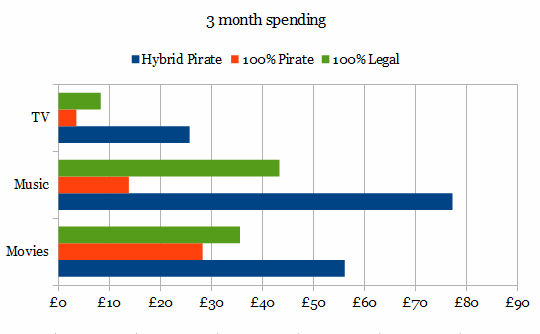
\includegraphics[width=\textwidth]{images/budget-culture.png}
{\footnotesize Source : \url{http://torrentfreak.com/uk-movie-pirates-spend-way-more-at-the-box-office-121122/}}
\caption{Budget culture/divertissement des internautes anglais}
\end{figure}

On remarque que ce sont à chaque fois les internautes <<~hybrides~>> qui vont le plus dépenser, et non pas, comme on pourrait le croire, ceux qui empruntent uniquement le chemin de la légalité.

Ces deux études convergent vers une conclusion similaire : le libre partage des œuvres ne tue pas la création, au contraire.

Il faut voir que les nouvelles technologies numériques ont rendu quasiment obsolètes les industries de la culture.
Ce sont des choses qui sont déjà arrivées, et qui arriveront encore.
Laissez-moi vous parler des vendeurs de glace \dots{}\footnote{Source : \url{http://reformedroitauteur.sploing.fr/\#htoc93}}

Il y a 100 ans, la compagnie <<~Stockholm Is~>> était l'un des plus importants employeurs de Stockholm en Suède.
Leur commerce était aussi simple que nécessaire : aider à conserver les denrées périssables plus longtemps en distribuant du <<~froid~>> dans un format adéquat.

Pour cela, ils découpaient durant l'hiver de grands blocs de glace sur les lacs gelés, les conservaient dans des granges sur de la sciure, coupaient les blocs en de plus petits morceaux et les revendaient dans la rue. Les gens achetaient alors la glace et l'entreposaient avec la nourriture dans des placards spéciaux, les aliments étaient ainsi conservés au frais.

Au cours de la première moitié du siècle dernier, les foyers de Stockholm furent équipés de l'électricité.
Ces revendeurs de froid devinrent ainsi obsolètes.
Après tout, ce qu'ils proposaient n'était rien d'autre que la possibilité de conserver la nourriture au frais, et à présent tout le monde en était capable.

Ce fut un processus assez rapide dans les villes.
Avec la disponibilité du réfrigérateur à partir de 1920 environ, la plupart des foyers acquirent le leur à la fin des années trente.
L'un des plus importants employeurs de la ville devint complètement obsolète à cause d'une avancée technique.

Il y eu de nombreuses tragédies personnelles à cette époque du fait que les vendeurs de glace perdirent leur gagne pain et durent se former afin de retrouver un emploi dans un nouveau secteur. Les vendeurs de glace ont souvent eu du mal à se reconvertir, et voir leur secteur se désintégrer à toute vitesse ne les a pas aidé.

Voici quelques faits qui n'ont pas eu lieu lorsque l'industrie de distribution de glace devint obsolète :

\begin{itemize}
\item Aucun propriétaire de réfrigérateur ne fut poursuivi en justice pour <<~production de son propre froid~>>, ignorant ainsi les sociétés de distribution de froid.
\item Aucune loi ne fut proposée pour rendre les compagnies d'électricité passibles de poursuites dans le cas où l'électricité qu'elles fournissaient aurait été utilisée d'une manière pouvant porter préjudice au travail de vendeur de glace.
\item Personne ne demanda une taxe mensuelle aux propriétaires de réfrigérateur au profit du syndicat des vendeurs de glace.
\item Il n'y a pas eu de prolifération de coûteux panels d'experts pour soutenir combien les vendeurs de glace étaient importants pour l'économie toute entière.
\end{itemize}

\textit{Oui, ce sont des choses qui sont arrivées de nos jours \dots{}}

Par contre, la distribution monopolistique devint obsolète et l'économie en général bénéficia de cette décentralisation.

On apprend de l'histoire, qu'à chaque fois qu'une industrie devient obsolète, cela est bénéfique.
Cela traduit que l'on a appris quelque chose d'important : faire les choses d'une manière plus efficace.
De nouvelles compétences et de nouveaux secteurs industriels apparaissent toujours dans leurs sillages.

Les industries actuelles devraient s'adapter au progrès, et pas tenter d'adapter le progrès à leurs modèles économiques vieillissants.
Je pense que nous sommes à l'aube d'une révolution : celle de l'industrie de la culture et de la question du partage des œuvres de l'esprit.

Il faut réinventer des modèles économiques qui profitent aux créateurs et à ceux qui ajoutent de la valeur.
C'est encore une fois une problématique complexe, d'autant que, cette fois-ci, il faut penser ces modèles dans une logique d'abondance et non plus de rareté.
Certaines idées ont déjà émergé, mais toutes ne sont pas bonnes.
\textit{L'exemple qui va suivre est très inspiré du chapitre 6 du document <<~Sur la réforme du droit d'auteur~>>\footnote{\url{http://reformedroitauteur.sploing.fr/}}.}

La licence globale, par exemple, est un forfait illimité pour la culture sous forme d'une taxe sur l'Internet haut débit.
C'est une idée qui est dans l'air du temps depuis au moins une décennie, mais n'est jamais devenue réalité.
L'idée semble simple et éventuellement attractive au premier abord, mais lorsque l'on commence à s'intéresser aux détails afin de formuler une proposition concrète, on prend conscience des problèmes.

Collecter l'argent est une chose. On peut discuter pour savoir si c'est juste d'obliger les gens qui ne téléchargent rien à payer quand même, ou pour savoir pourquoi des entreprises devraient être dédommagées pour cause de progrès technologique, ou encore pour savoir comment prendre en compte les multiples connexions à Internet que possède une famille.
Mais laissons cela de côté.
C'est lorsque l'on se demande comment l'argent devrait être réparti que les choses amusantes commencent.

Si l'on calcule les gains des artistes sur base de ce qui est joué à la télévision et la radio, la plupart de l'argent va aller aux artistes établis qui gagnent déjà très bien leur vie.
C'est la manière dont fonctionne le système actuellement avec les prélèvements sur les supports vierges et les appareils électroniques.
L'une des caractéristiques les plus intéressantes d'Internet, c'est le fait que les plus petites performances confidentielles peuvent atteindre leur public, même si elles ne sont pas jouées à la télévision et la radio. L'addition de toutes les petites performances constitue une part importante de ce qui est téléchargé sur le net.

Ces petits artistes sont ceux que la plupart des gens souhaitent supporter, à la fois pour la diversité culturelle qu'ils assurent, et simplement parce que très souvent ils ont vraiment besoin de ces revenus.
Avec un forfait basé sur la diffusion à la télévision et la radio, ils n'obtiendraient qu'une très faible partie de l'argent collecté.
Dans le même temps, leurs fans disposeraient de moins de ressources financières pour supporter ces artistes, puisqu'ils auront déjà dû payer le forfait.
L'effet immédiat serait un système qui diminue les revenus des artistes pauvres et distribue l'argent à ceux qui sont déjà riches.

Une alternative, préférée par le plus grand nombre des partisans de la licence globale, est au contraire de mesurer ce qui est partagé sur internet et de baser les gains aux artistes sur ces mesures. Mais cela engendre d'autres problèmes.

35\% des téléchargements sur Internet sont de la pornographie\footnote{Source : \url{http://www.numerama.com/magazine/16005-la-pornographie-occupe-un-tiers-du-web-selon-une-societe-specialisee-dans-le-filtrage.html}}.
L'industrie pornographique possède exactement la même protection du droit d'auteur que les autres productions audiovisuelles.
Si les paiements d'un forfait culturel sont considérés comme un <<~dédommagement~>> pour le téléchargement d'œuvres protégées par le droit d'auteur, alors 35\% de l'argent devrait immédiatement reversé à l'industrie pornographique.

Le point ici n'est pas de critiquer la pornographie en tant que telle.
Mais ça ne veut pas dire qu'elle ait besoin de milliards provenant de subventions gouvernementales.
Au cours de l'histoire, c'est une industrie qui a démontré sa capacité à s'adapter de son propre chef.

Si on veut exclure la pornographie, on ne pourra plus dire que la licence globale rémunère les artistes qui sont appréciés, ou alors il faudra inventer une organisation qui aurait pour but de décréter où se situe la limite entre art et pornographie \dots{}

Il est techniquement possible de mesurer ce qui est partagé sur Internet avec une précision relativement élevée.
Mais à la minute à laquelle on commencera à rémunérer suivant des statistiques de téléchargement, les gens changeront de comportement.
Aujourd'hui, si on aime un artiste qui a produit un nouvel album, on le télécharge pour pouvoir l'écouter.
Mais si on savait que notre artiste préféré gagnera de l'argent en proportion de nos téléchargements, nous le retéléchargerons sans cesse pour l'aider.
Ainsi, Internet sera en permanence congestionné par du trafic inutile, peu importe la capacité ajoutée par les opérateurs.

Autre point, les virus sont aujourd'hui un problème majeur, malgré qu'il soit assez difficile pour leurs créateurs de les rentabiliser.
Le but d'un virus est généralement d'installer une porte dérobée dans l'ordinateur, pour que celui-ci devienne part d'un réseau d'ordinateurs vérolés, un botnet, que le créateur du virus peut contrôler à sa guise.
Le détenteur d'un botnet peut vendre ses services à des organisations criminelles qui veulent envoyer du spam ou commettre diverses formes de fraude, mais à moins qu'il ait des liens avec le crime organisé, il n'est pas facile pour lui de rentabiliser ses talents.
Avec une licence globale, tout change.

Chaque propriétaire d'un botnet n'aurait comme seul besoin celui d'avoir un ami qui a enregistré une chanson couverte par le droit d'auteur.
Ses milliers d'ordinateurs sous contrôle n'auront qu'à télécharger sans répit cette chanson.
Grâce à la licence globale, ces téléchargements généreront automatiquement des revenus pour son ami.
Pour les formes de fraude les plus simples, la police arrivera peut-être à détecter son activité criminelle et à y mettre fin, mais on peut facilement imaginer que des systèmes de fraude sophistiqués verront le jour.
La licence globale deviendrait donc une excellente source de revenu pour les criminels, pour les éditeurs de virus.

La licence globale n'est donc pas une solution viable.
Mais surtout, elle répond à des problèmes qui n'existent pas !

Internet est une technologie révolutionnaire qui change la plupart des présuppositions de l'industrie de la culture.
La tâche des politiques n'est pas de protéger les vieux modèles économiques ou d'en inventer de nouveaux.
Ils doivent seulement s'assurer que la société dans laquelle nous vivons puisse être florissante et que les gens créatifs puissent vivre de ce qu'ils font.

C'est pour cette raison que je l'affirme : il faut valoriser les créateurs.

%(les pirates achètent, inutilité licence globale, inventer des modèles économiques, exemple des vendeurs de glace)
\section{La réforme du système actuel}

On assiste donc à une véritable lutte des pouvoirs.
Les industries de la culture sont en train d'essayer de freiner le progrès pour engendrer plus de profit.
Elles n'hésitent pas à faire du lobbying auprès de nos politiques qui semblent, pour la plupart, dépassés par ces problématiques.

Heureusement, il existe un parti politique qui traite ces problèmes et qui commence doucement à s'implanter en Europe et dans le monde entier : le Parti pirate.

Le Parti pirate s'attache notamment à réformer les droits de la propriété intellectuelle et à soutenir ou renforcer les droits fondamentaux relatifs à la vie privée.
Le programme du parti se concentre sur ce sujet transversal et il n'est donc pas possible d'attribuer au Parti pirate une position de droite ou de gauche.

Ce parti est un phénomène mondial : il existe des Partis pirates dans de nombreux pays à travers le monde.
Ceux-ci sont des entités indépendantes les unes des autres, mais sont reliés par le Parti pirate international.

À l'origine, le premier Parti pirate fut créé en Suède, mais le mouvement a également été représenté lors d'élections en Allemagne et en France\footnote{Voir leur site : \url{http://www.partipirate.org/}}.

Voici donc les réformes du droit d'auteur que propose le Parti pirate :

\paragraph{Mesure 1}
\textit{Personne ne devrait être autorisé à déclarer qu'il est Paul Mc Cartney s'il ne l'est pas.
Ce devrait être illégal.
<<~Rendre à César ce qui est à César >> est une maxime qui met tout le monde d'accord.}

Dans les faits, c'est un concept qui est très bien appliqué sur Internet.
Les blogueurs ont tendance à citer leurs sources d'une façon qui fait bien plus que respecter le minimum légal.
Il y a plusieurs raisons à cela.
Cela rend leur blogue plus crédible s'ils donnent les liens vers leurs sources afin que leurs lecteurs puissent en vérifier l'origine s'ils le souhaitent.
Les personnes qu'ils citent sont contentes, elles seront donc plus enclines à citer les blogues en question si l'occasion s'y présente, et ceux-ci verront leur trafic augmenter.
Voilà les raisons pratiques pour lesquelles il est dans l'intérêt d'un blogueur d'être plus généreux au niveau des citations de ses sources que ne l'exige aucune loi.

Le droit d'être reconnu en tant qu'auteur sur Internet n'est pas menacé.
Le Parti pirate propose donc de laisser inchangé ce point de la législation du droit d'auteur.

\paragraph{Mesure 2}
\textit{Nous voulons que le droit d'auteur redevienne ce pourquoi il a été conçu, et rendre clair qu'il ne doit réguler que les échanges commerciaux. Copier ou utiliser un travail protégé sans but lucratif ne devrait jamais être interdit.
Le pair à pair est, entre autres, une bonne raison pour cette légalisation.}

Pour eux, une telle avancée est :

\begin{itemize}
\item inéluctable : la limitation du partage de fichiers par les lois et la répression ne fonctionnent pas, et sont contournées.
\item indispensable : les tentatives d'imposer l'interdiction du partage de fichiers mettent en danger les droits fondamentaux.
\item inoffensive : les artistes et le secteur de la culture, dans leur ensemble, se portent bien malgré le partage de fichiers (ou peut être grâce à lui), il n'y a donc pas de réel problème à résoudre.
\item facile à mettre en place : <<~Suivre l'argent~>> suffit aux autorités pour leur permettre de garder une trace des activités commerciales.
\end{itemize}

\paragraph{Mesure 3}
\textit{Nous souhaitons raccourcir les durées de protection à quelque chose de raisonnable à la fois du point de vue de la société et des investisseurs, et nous proposons 20 années à partir de la publication.
Nous souhaitons la même période de protection pour tous les types de création.}

On pourrait se dire qu'il serait intéressant d'adapter la durée de la protection au type d'œuvre auquel on a affaire.
Malheureusement il s'avère en pratique difficile de trouver un compromis, les avis divergeant énormément en fonction des sensibilités de chacun.

De plus, dans la plupart des projets culturels sérieux, on attend que le projet s'autofinance et commence à dégager des bénéfices au bout de quelques années, grand maximum.
Ces projets n'ont pas besoin d'une protection de la durée d'une vie, étant donné qu'ils sont prévus par les investisseurs pour être rentabilisés en quelques années.

\paragraph{Mesure 4}
\textit{La protection du droit d'auteur devrait être accordée automatiquement dès la publication comme aujourd'hui, mais si les propriétaires veulent continuer à jouir de leurs droits après les cinq premières années de publication, ils devraient se manifester de sorte qu'ils soient facilement trouvables.}

J'en parlais précédemment (page \pageref{oeuvres-orphelines}), le problème des œuvres orphelines est bien réel.
Environ 75\% des livres que Google souhaite numériser dans le cadre de leur <<~Google Books initiative~>> sont épuisés, mais toujours sous droits d'auteur.
Même s'il est théoriquement possible de retrouver le détenteur des droits pour beaucoup de ces livres en entreprenant une investigation pour chaque cas individuel, cela devient en pratique infaisable lorsqu'on veut numériser en masse.

Ce que propose le Parti pirate, c'est que si on désire une rémunération pour l'usage d'une de nos œuvres plus vieille que 5 ans, on doit faire savoir auprès d'une base de données publique comment être contacté et où faire parvenir l'argent.

\paragraph{Mesure 5}
\textit{Nous voulons changer la situation en introduisant des exceptions claires de droit au remix ou à la parodie, de même que de droits de citation pour les matériaux audiovisuels qui se calquent sur la législation existante pour les textes.}

Peut on être propriétaire d'un son ? 
Aujourd'hui, la réponse à cette dernière question est malheureusement oui.
Les majors revendiquent la propriété sur des sons individuels et de très courts extraits.
Si on est un musicien hip-hop, il faut s'attendre à payer des centaines de milliers d'euros par avance pour avoir le droit d'utiliser des samples si on souhaite toujours rendre sa musique accessible au public \dots{}

C'est clairement une restriction du droit de créer de nouvelles cultures.

\paragraph{Mesure 6}
\textit{Il devrait être systématiquement légal de passer outre les MTP\footnote{MTP = DRM ; j'en parle page \pageref{drm}} et nous devrions bannir les MTP qui empêchent des usages légaux.
Les grandes multinationales ne devraient pas avoir le droit d'écrire leurs propres lois d'utilisation des fichiers.}

J'ai déjà évoqué ce thème, assez largement je pense pour convaincre de sa nocivité pour la création.

\vspace{50pt}

Il faut garder en tête que si ces réformes constituent un objectif, la plus difficile sera de trouver le chemin le moins tortueux pour y arriver.
J'espère vraiment que les bonnes personnes seront mises au pouvoir bientôt, car il est urgent de réformer le droit d'auteur.
Aucun modèle économique ne vaut mieux que nos droits civiques.

% état final != transition
%(lutte de pouvoirs, propositions du parti pirate)

\chapter*{Conclusion}
\addcontentsline{toc}{chapter}{Conclusion}

Nous avons vu qu'il n'est pas vraiment possible de dissocier les actions de créer et de copier.
La copie est quelque chose que nous faisons tous les jours, y compris lorsque nous apprenons.
Nous sommes nous-mêmes littéralement le résultat d'une copie : celle de nos cellules.
Les idées, et autres œuvres de l'esprit, ne fonctionnent pas comme de simples objets, et ne peuvent pas vraiment être compatibles avec la notion de propriété.

Cependant, la société actuelle continue de maintenir les systèmes du brevet et du droit d'auteur.
Ces systèmes n'ont eu que peu de légitimité depuis leur création, et sont aujourd'hui complètement décalés par rapport à une réalité d'œuvres de plus en plus numériques.
La copie ne devrait pas être interdite, mais devrait au contraire être encouragée dans une démarche gagnant- gagnant.
Sinon, aller jusqu'au bout de son interdiction reviendrait à instaurer un état totalitaire, où l'espionnage des citoyens est fait de manière massive.

Heureusement, le futur s'éclaircit sur ce point.
La philosophie du libre est peut être l'un des moyens de rédemption du système actuel.
Elle permet de ne pas devenir esclave du progrès et de nos propres machines, en confiant le pouvoir aux utilisateurs et non pas aux créateurs.
Cet état d'esprit a montré au fil des années qu'il était source d'une grande et saine créativité (il suffit de voir, par exemple, le nombre d'inventions ingénieuses réalisées par des enfants et basées sur des cartes Arduino\footnote{Carte électronique programmable et <<~open hardware~>>\\Voir \url{http://arduino.cc/fr/Main/DebuterIntroduction}}).

Mon opinion est qu'il est important de soutenir les logiciels libres.
Bien évidemment, il est possible pour ça de donner bien des choses : ses compétences, son temps, son implication, des ressources \dots{}

Mais il est aussi possible de faire bien plus simple : de les utiliser et d'en parler.
Il existe en effet d'excellents logiciels libres, que j'utilise personnellement tous les jours.
On peut citer \href{https://www.mozilla.org/fr/firefox/new/}{Mozilla Firefox}, \href{https://www.mozilla.org/fr/thunderbird/}{Mozilla Thunderbird}, \href{https://www.videolan.org/vlc/}{VLC}, \href{http://fr.libreoffice.org/}{LibreOffice}, \href{http://www.gimp.org/}{GIMP} et même certains contenus en ligne majeurs comme \href{https://fr.wikipedia.org/}{Wikipédia} ou \href{http://www.openstreetmap.org/}{OpenStreetMap}.
Plus ces logiciels seront utilisés, plus ils gagneront en crédibilité et pourront nous protéger contre leurs alternatives propriétaires qui nous délestent progressivement de nos droits fondamentaux.

La solution se trouve aussi du côté du Parti pirate.
Peu m'importe si celui-ci arrive au pouvoir ou pas, tant que les idées qu'il véhicule sont mises en œuvre.
Pour l'heure, le moyen le plus simple est de le faire monter en puissance, et de le soutenir.
J'y penserai sérieusement si j'ai un jour l'occasion de voter pour un de ses représentants.
Et j'espère que ce jour arrivera bientôt.

Ami lecteur, si toi aussi tu veux un monde meilleur, tu sais ce qu'il te reste à faire.

% soutenir le libre

\appendix

\chapter{Violations de brevet dans le domaine des smartphones}
\label{annexe-smartphones}

Source : \url{http://visual.ly/tech-patent-wars}

\newpage

\begin{figure}[H]
\center
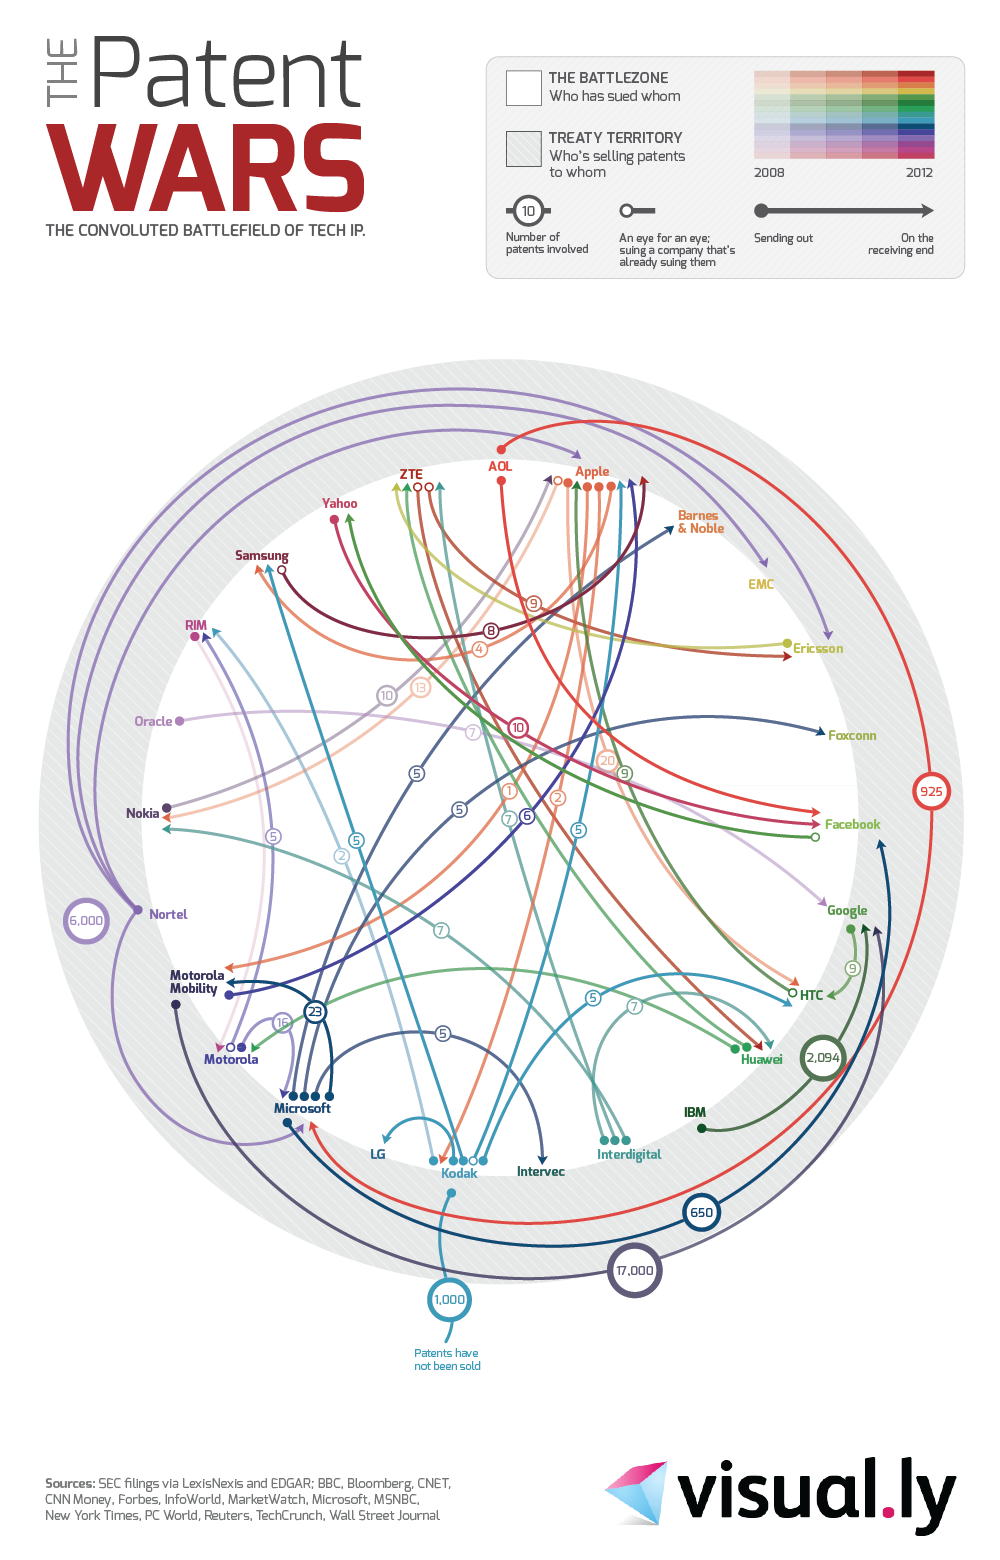
\includegraphics[width=0.9\textwidth]{images/patent-wars.png}
\caption{Violations de brevet dans le domaine des smartphones}
\end{figure}

\chapter{DVD piraté vs. DVD acheté}
\label{annexe-dvd}

Source :\\
\url{http://bugbrother.blog.lemonde.fr/2010/02/22/le-fbi-menace-les-acheteurs-de-dvd/}

\newpage

\begin{figure}[H]
\center
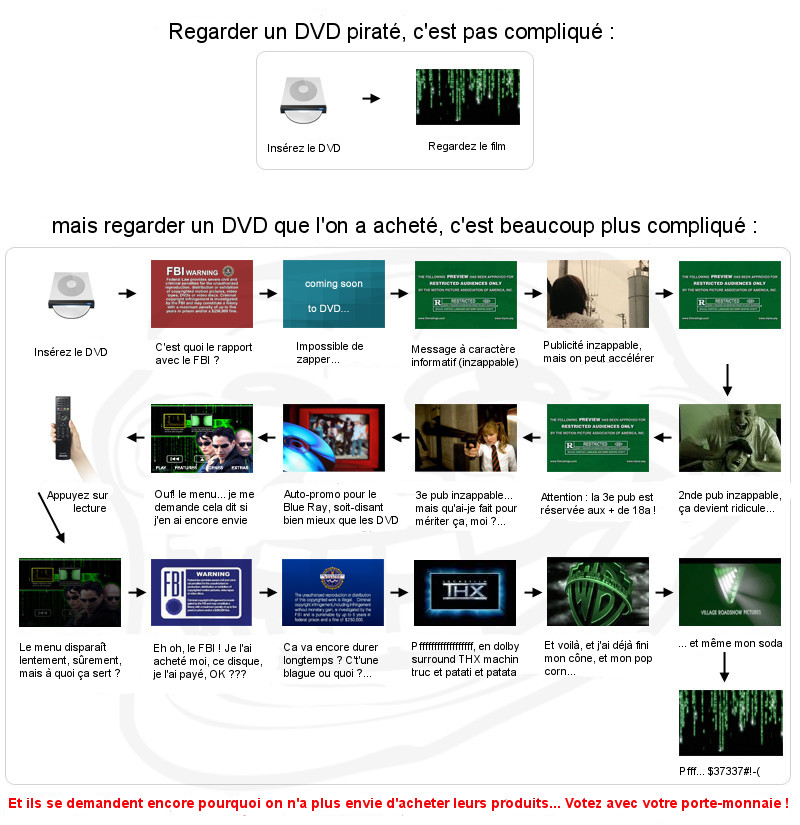
\includegraphics[width=\textwidth]{images/dvd-legal-dvd-illegal.jpg}
\caption{DVD piraté vs. DVD acheté}
\end{figure}

\chapter{Mon vélo, de Marcel-André Casasola Merkle}
\label{annexe-velo}

Cette traduction est une analogie qui aide à comprendre les abus et dangers du contrôle des œuvres.

Source de la traduction (licence CC-BY-SA) :\\
\url{http://reformedroitauteur.sploing.fr/\#htoc109}

Source du texte original (licence CC-BY) :\\
\url{http://www.137b.org/?p=2445}

\newpage

Je me suis acheté un vélo. Un beau modèle. Je l’ai attendu longtemps.

Aux États-Unis, ça fait déjà longtemps qu’il est sur le marché. Pas en Allemagne. Et l'importer aurait été illégal. Le mois dernier, on pouvait le louer auprès d'une grande chaîne de télé pendant une semaine et faire une virée. Ça m'a plu.

Mais à la fin de la journée, il était de nouveau verrouillé. Et je devais attendre.

Par la suite, le vélo est devenu disponible dans les arrières-cours de mon quartier pour pas un rond. Ça m'a paru un peu louche.

Mais je m'en fiche. Maintenant, j'ai mon vélo. Et il est beau.

Il est marqué jusque sur les autocollants du cadre que je ne dois pas voler ou reconstituer de vélo. Logique. Pourquoi d'ailleurs ? Je l'ai bel et bien acheté.

Avant le premier démarrage, j'ai dû appeler le fabricant et lui expliquer quels étaient les trois quartiers de la ville dans lesquels je voulais utiliser mon vélo. Lorsque je circule dans un quartier non autorisé, les freins s'enclenchent tout seul. Je n'ai rien à faire. Ça fait partie du service. Je peux alors appeler le fabricant et reconfigurer le vélo. De la sorte je circule dans toute la ville.

Si je voulais louer mon vélo, ça ne me serait pas permis. La selle envoie des petites décharges dans le corps et signifie son désaccord. C'est à la répartition des masses à l'arrière qu'elle reconnaît qui s'assoit sur le vélo. Et si ce n'est pas moi, la sonnette carillonne. Du coup, je fais attention à mon régime. Sinon mon vélo ne me reconnaît plus.

Il y a peu, j'ai voulu le repeindre. Je trouvais que le kaki faisait vieux jeu. En grande surface on m'a ri au nez. Ça serait tout à fait illégal. Est-ce que j'avais demandé au fabricant ? Il aurait sûrement dû prévoir quelque chose pour la couleur.

La ville vient de construire de nouvelles pistes cyclables et je trouvais qu'elle avait raison. Mais j'ai entendu une rumeur : Mon vélo ne peut plus rouler dessus. Les pneus sont trop minces. Ils ne passent plus sur le nouveau revêtement.

Mais une nouvelle génération arrive. Avec des chenilles. Ils seront beaucoup plus sûrs.

Et maintenant, il y a des postes de police sur les pistes. Pour contrôler qui est sur quel vélo. Et quand on perd le contact visuel avec tous les postes, le vélo éjecte son passager. Par temps de brouillard on voit souvent des hommes joncher la route comme des fruits trop mûrs.

Si on me vole mon vélo, ça peut devenir encore plus cher. Parce qu'en effet je l'ai diffusé. Le constructeur ne peut plus en vendre un directement au voleur. Et j'en suis responsable.

Tout ça m'est devenu trop périlleux. Maintenant je veux donner mon vélo à d'autres. Mais on chuchote que ce ne serait pas permis. Mon vélo ne serait qu'à moi. Je l'ai donc simplement supprimé.


\listoffigures

\end{document}